\section{Introduction}

% --- Slide 1: The Challenge ---
\begin{frame}{The Challenge: Can a Neural Network Play Pac-Man?}

	The goal of this project is to train an artificial neural network to master the classic arcade game, Pac-Man.
	This non-trivial task requires the agent to develop complex strategies for:

	\begin{minipage}{0.55\textwidth}

		\vspace{0.5em}
		
		\begin{itemize}
			\item Efficient maze navigation
			\item Dynamic evasion of multiple, intelligent opponents (ghosts)
			\item Strategic use of resources (power-ups)
			\item Long-term planning to clear the entire level
		\end{itemize}
		
		\vspace{1em}
	\end{minipage}%
	\hfill
	\begin{minipage}{0.45\textwidth}
		\centering

		\vspace{-0.5em}

		\begin{figure}
			\centering
			\includegraphics[width=0.82\linewidth]{assets/maze.png} % Usa una tua immagine di Pac-Man
			
			\vspace{-1em}

			\caption{\centering \small Pac-Man environment}
		\end{figure}

		\vspace{-1em}
	\end{minipage}

	Instead of traditional programming, we use an evolutionary approach to \textbf{discover} these strategies automatically.
\end{frame}

% --- Slide 2: Our Tool: NEAT ---
\begin{frame}{Our Tool: NeuroEvolution of Augmenting Topologies}
		We use \textbf{NEAT} \cite{stanley2002evolving}, a powerful algorithm that evolves both the \textbf{weights} and the \textbf{structure (topology)} of neural networks.

		Key features of NEAT:
		\begin{itemize}
			\item \textbf{Complexification:} Starts with simple networks and gradually adds nodes and connections.
			\item \textbf{Innovation Numbers:} Tracks the historical origin of genes to solve the "competing conventions problem" during crossover.
			\item \textbf{Speciation:} Groups similar networks to protect new innovations until they're ready to compete.
		\end{itemize}

		\vspace{-1em}
		
		\begin{figure}
			\centering
			\includegraphics[width=0.5\linewidth]{assets/neat-evolution.png}
			\vspace{-1em}
			\caption{NEAT increases network complexity over time \cite{shrestha2025reinforced}.}
		\end{figure}

\end{frame}

% --- Slide 3: Project Architecture ---
\begin{frame}{Project Architecture}
	The project integrates the NEAT algorithm with a custom Pac-Man game environment.
	
	\vspace{0.5em}

	\begin{columns}[T]
		\begin{column}{0.5\textwidth}
			\textbf{Pac-Man Game Engine}
			\begin{itemize}
				\item Adapted from the \textit{PyPacman} repository.
				\item Refactored game state management for stability and performance in a machine learning context.
				\item Core logic encapsulated in a Gym-like environment.
			\end{itemize}
		\end{column}
		\begin{column}{0.5\textwidth}
			\textbf{NEAT Framework}
			\begin{itemize}
				\item \texttt{trainer.py}: Manages the evolutionary loop, population, and checkpoints.
				\item \textbf{Parallel Evaluation:} Uses Python's multiprocessing to evaluate hundreds of genomes simultaneously, drastically reducing training time.
			\end{itemize}
		\end{column}
	\end{columns}
	
	\begin{figure}
	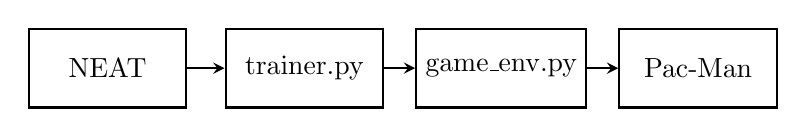
\begin{tikzpicture}[node distance=2.5cm, >=stealth, thick]
		\node (neat) [draw, rectangle, minimum width=2cm, minimum height=1cm] {NEAT};
		\node (trainer) [draw, rectangle, minimum width=2cm, minimum height=1cm, right of=neat] {trainer.py};
		\node (game_env) [draw, rectangle, minimum width=2cm, minimum height=1cm, right of=trainer] {game\_env.py};
		\node (pacman) [draw, rectangle, minimum width=2cm, minimum height=1cm, right of=game_env] {Pac-Man};
		\draw[->] (neat) -- (trainer);
		\draw[->] (trainer) -- (game_env);
		\draw[->] (game_env) -- (pacman);
	\end{tikzpicture}
	\caption{High-level interaction between NEAT and the game environment.}
	\end{figure}
\end{frame}

\begin{frame}{Choosing a Game Environment}
	
	To train and evaluate NEAT agents, a reliable Pac-Man environment was essential. After surveying available options, I selected the \textit{PyPacman} repository~\cite{pypacman} for its simplicity and open-source nature.

	\vspace{0.5em}
	\begin{columns}[T]
		\begin{column}{0.48\textwidth}
			\textbf{Advantages:}
			\begin{itemize}
				\item Lightweight and easy to understand
				\item Fully open-source and modifiable
				\item Minimal dependencies
			\end{itemize}
			\textbf{Why this matters:}
			\begin{itemize}
				\item Fast simulation of thousands of games per generation
				\item Easy integration with custom agent logic
			\end{itemize}
		\end{column}
		\begin{column}{0.48\textwidth}
			\textbf{Limitations:}
			\begin{itemize}
				\item Contained several bugs and inconsistencies
				\item Not optimized for large-scale, automated runs
			\end{itemize}
			\textbf{Actions Taken:}
			\begin{itemize}
				\item Refactored core game logic for stability and speed
				\item Added a Gym-like interface for agent-environment interaction
			\end{itemize}
		\end{column}
	\end{columns}

	The repository provided a solid foundation, but required several changes to meet the needs of this project.

\end{frame}